% This template was initially provided by Dulip Withanage.
% Modifications 
% were made by Conny Junghans and Jannik Strötgen
% and Sascha Hunold

\documentclass[
     12pt,                    % font size
     a4paper,             % paper format
     BCOR10mm,     % binding correction
     DIV14,                 % stripe size for margin calculation
     listof=totoc,                    % table listing in toc
     bibliography=totoc,       % bibliography in toc
     index=totoc,              % index in toc
%     parskip            % paragraph skip instead of paragraph indent
     twoside,
     headsepline
     ]{scrreprt}

%%%%%%%%%%%%%%%%%%%%%%%%%%%%%%%%%%%%%%%%%%%%%%%%%%%%%%%%%%%%


% PACKAGES:

% Use German :
% make sure texlive-lang-german is installed (for TexLive)
\usepackage[ngerman,english]{babel}
% Input encoding
\usepackage[utf8]{inputenc}
% Font encoding
\usepackage[T1]{fontenc}
% Index-generation
\usepackage{makeidx}
% Einbinden von URLs:
\usepackage{url}
% Special \LaTex symbols (e.g. \BibTeX):
\usepackage{doc}
\usepackage[backend=bibtex,sorting=ynt]{biblatex}
% Include Graphic-files:
\usepackage{graphicx}

% Fuer anderthalbzeiligen Textsatz
\usepackage{setspace}

% hyperrefs in the documents
\usepackage[bookmarks=true,colorlinks,pdfpagelabels,pdfstartview = FitH,bookmarksopen = true,bookmarksnumbered = true,linkcolor = black,plainpages = false,hypertexnames = false,citecolor = black,urlcolor=black]{hyperref} 

\usepackage{amsmath}
\usepackage[nameinlink]{cleveref}
\usepackage[table]{xcolor}
\usepackage{booktabs}
\usepackage[chapter]{minted}
\definecolor{LightGray}{gray}{0.9}

\usepackage[separate-uncertainty = true, separate-uncertainty-units = repeat]{siunitx}

\usepackage{pgfplots}
\pgfplotsset{width=10cm, compat=1.9}

\usepgfplotslibrary{external}
\tikzexternalize


%%%%%%%%%%%%%%%%%%%%%%%%%%%%%%%%%%%%%%%%%%%%%%%%%%%%%%%%%%%%

% OTHER SETTINGS:

% Pagestyle:
\pagestyle{headings}

% Choose language
\newcommand{\setlang}[1]{\selectlanguage{#1}\nonfrenchspacing}

\addbibresource{references}

\begin{document}

% TITLE:
\pagenumbering{roman} 
\begin{titlepage}

\setlang{ngerman}

\vspace*{1cm}
\begin{center}
\vspace*{3cm}
\textbf{ 
\Large Ruprecht-Karls-Universität Heidelberg\\
\smallskip
\Large Institut für Informatik\\
\smallskip
\Large Artificial Intelligence for Programming\\
\smallskip
}

\vspace{3cm}

\textbf{\large Bachelorarbeit} % Studienarbeit, Interdisziplinaeres Projekt

\vspace{0.5\baselineskip}
\huge
\setlang{english}
PandaRec - Code Recommendation System for the Pandas Library based on Recipes \\
\vspace{0.5\baselineskip}
\setlang{ngerman}
PandaRec - Code-Empfehlungssystem für die Pandas-Bibliothek auf Basis von Rezepten

\end{center}

\vfill 

{\large
\begin{tabular}[l]{ll}
Name: & Frederick Vandermoeten\\
Matrikelnummer: & 4055264\\
Betreuer: & Prof. Dr. Artur Andrzejak\\
Datum der Abgabe: & 19.10.2023
\end{tabular}
}

\end{titlepage}

\onehalfspacing

\thispagestyle{empty}

\vspace*{100pt}
\noindent
Ich versichere hiermit, dass ich diese Bachelor-Arbeit selbstständig verfasst und keine anderen als die angegebenen Hilfsmittel benutzt habe.
Sowohl inhaltlich als auch wörtlich entnommene Inhalte wurden als solche kenntlich gemacht.
Die Arbeit ist in gleicher oder vergleichbarer Form noch bei keiner andere Prüfungsbehörde eingereicht worden.

\vspace*{50pt}

\noindent
Heidelberg, dd.mm.yyyy
\cleardoublepage

\section*{Zusammenfassung}

Dies ist eine Zusammenfassung der Arbeit.

\setlang{english}
\section*{Abstract}

This is the abstract.

\tableofcontents
\cleardoublepage
\pagenumbering{arabic} 

% List of figures (Abbildungsverzeichnis):
\listoffigures
% List of tables (Tabellenverzeichnis):
\listoftables

\listoflistings
\cleardoublepage

%%%%%%%%%%%%%%%%%%%%%%%%%%%%%%%%%%%%%%%%%%%%%%%%%%%%%%%%%%%

\chapter{Introduction}\label{intro}

\section{Motivation}

(NOTE: title page has institut in german and lehrstuhl in english, ask prof what i should write)

Pandas is a library for Python that provides data analysis and manipulation tools~\cite{pandaswebsite}. While it is powerful and flexible, it is equally complex.

Researchers from all fields often have to work with data. However, researchers or users new to data analysis can struggle to learn how to use pandas or similar data manipulation software since searching documentation and tutorials is time-intensive. If the user has limited programming knowledge, this problem gets exacerbated since they must learn multiple things simultaneously.

Code recommendation systems are a staple in modern software development. Different methods can help developers write code faster and more efficiently, increase code clarity and maintainability, and help with error detection.

\section{Problems}

A recommendation system for the pandas library should be fast, easy to set up, easy to use, and useful to all users. That means it should provide the user with relevant recommendations even if they still need to gain domain knowledge. However, current code recommendation only fulfill some of the described requirements.

\section{Solutions}

My solution uses a Jupyter Notebook GUI that anyone can easily set up in the browser. I will use a set of "recipes" code snippets with at least a name and a description.

In the pursuit of developing a sound code recommendation system, we will compare different methods of recommending code and implement them modularly so that methods can be easily exchanged and even composed out of multiple methods.

\section{Structure of this Thesis}

In the second chapter, I will present the current state of recommendation systems for pandas and the techniques that I will use in my recommendation system.
The third chapter deals with the design of the GUI and modular recommendation system and then the implementation of the recipes and different algorithms.
In the fourth chapter, I will evaluate how the specific ranking algorithms and the different recipe datasets perform compared to each other and other recommendation systems.

\chapter{Background}\label{background}

This chapter will introduce the needed background knowledge to the reader. It will introduce the Pandas library, Code Recommendation Systems, how to search for code, and how to rank our recommendation algorithms. 

\section{Pandas}

Pandas is an open-source library for the Python programming language that provides data analysis and manipulation tools. The core of the library are the Series and DataFrame data structures. Series are one-dimensional labeled arrays of any type. DataFrames are two-dimensional data structures that function like a table with rows and columns. Pandas provides tools for data cleaning, manipulation, analysis, and exploration of these data structures. Additionally, tools for data import and export are provided. Pandas also pairs well with visualization libraries like Matplotlib.

\section{Natural Language Processing (NLP)}

Natural language processing is a subfield of artificial intelligence that interprets and generates natural (human) language. In our specific case, we want to query in natural language since this is easier for a new user.

Let us look at existing recommendation systems so we can get an understanding of what our solution should be capable of.

\section{Code Recommendation Systems}\label{coderecsystems}

Code recommendation systems help developers write code more efficiently. They can suggest code snippets, highlight errors, and give quick access to documentation.
As described by
\citeauthor*{recommendationsystems}~\citeyear{recommendationsystems}~\cite{recommendationsystems}, code recommendation systems have these design dimensions:
\begin{description}
	\item[Context] is the input of the recommendation system. This can include a large amount of different information. We can look at what the user is typing, the file we are in, the codebase in general, and the interaction history. For pandas, we can also look at the current DataFrame and its column- and row names, datatypes, and with a GUI, what part of the DataFrame the user has highlighted.
	\item[The Recommendation Engine] uses the context and other data sources, such as data from different repositories and bug reports, to rank the recommendation output.
	\item[Output] can be provided either on demand or continuously and can be multiple suggestions or a single (often inline) suggestion.
	\item[User feedback] can change the system in many ways. The user can provide feedback by changing the context and adapting the recommendation engine locally or globally, where feedback either changes the output of the current user or all users.
\end{description}

\section{Existing Code Recommendation Systems}

The code recommendation system we want should be fast, easy to set up, use, and useful to all users.
So, let us look at a few existing code recommendation systems and see how they are inadequate for all our goals.

\subsection{Code Completion}

Code completion is already a part of most IDEs. It is a form of autocomplete. In its most usual form, after the user starts typing, it will recommend multiple completions of the typed word. While it helps to reduce typos, it cannot help a new user use a library since basic knowledge of the different functions is required. Code completion makes an experienced user more efficient, but more is needed for inexperienced users. Additionally, it requires an IDE, which will be an additional piece of software that someone who is unfamiliar with computer science would have to learn and set up.

\subsection{Code Generation}

Code recommendation systems can generate entire blocks of code. This can be used for boilerplate code or whole functions. While automated boilerplate cannot help with our use case, there are code generation systems that meet quite a lot of our requirements.

\subsection{Generative AI}

(NOTE: Maybe get rid of this, or move before semantic, or redo)
The Transformer~\cite{vaswani2017attention} has been shown to perform well on natural language processing tasks~\cite{radford2018improving}. Multimodal models like ChatGPT~\cite{chatgpt} and GitHub Copilot~\cite{copilot} are already commonly used to generate code. Using ChatGPT or GitHub Copilot by writing query-like comments performs decently on this task. Some problems are the cost of Copilot and the requirement to be online. How good they are will be discussed in the \Cref{evaluation}.

\section{Searching for Code}

Since my approach leverages "recipes", a corpus of common data manipulation tasks, I can use search algorithms to search through the descriptions of the recipes. Search algorithms that search for occurrences of the literal query are called lexical search algorithms.

\subsection{Lemmatization and Stemming}\label{lemmatize}

Since words can have different inflections, e.g., walked and walking, they need to be brought to a generic form. Stemming solves this by removing common suffixes. This can, however, result in stems that are not actual words. Lemmatization ensures that the resulting generic form is a valid dictionary entry. It requires linguistic knowledge and a complete vocabulary. Lemmatization is therefore more computationally intensive than stemming but provides more meaningful results.

\subsection{Lexical Search} \label{indexsearch}

In lexical search, the search engine looks for literal matches of the query words~\cite{bast2016semantic}.
A common and effective way to implement lexical search is with search indexing.

Search Indexing builds an inverted index out of the corpus. First, a forward index is built, which stores word occurrences per document. Then, the inverted index can be constructed, which stores for each word all the annotations that contain it~\cite{das2012indexing}.

With this index, the search algorithm can quickly retrieve a list of annotations containing the query.

\subsection{Semantic Search}\label{semantic}

Semantic search can be described as a search for meaning~\cite{bast2016semantic}. It aims to understand the meaning of a query instead of literal matches. The transformer~\cite{vaswani2017attention} is a deep learning architecture that can capture relationships between words and phrases, which enables context-aware applications. For this reason, transformer-based models such as the Generative Pre-trained Transformer~(GPT) and Bidirectional Encoder Representations from Transformers~(BERT) perform well on natural language tasks.

\subsection{Bidirectional Encoder Representations from Transformers (BERT)}

BERT~\cite{feng2020codebert} and the more extensively trained RoBERTa~\cite{liu2019roberta} are natural language processing models based on the transformer architecture. They were trained by predicting missing words (masked language model) in sentences from both left and right contexts (Bidirectional). This bidirectionality lends itself to sentence pair regression, like sentence similarity. With BERT, both sentences are passed into the model simultaneously, and the similarity is predicted. This is called cross-encoding and produces similarity scores with great accuracy. However, when cross-encoders compute the similarity between a query and a corpus, they will have to do a cross-encoding for every element of the corpus.

To combat this, Sentence-BERT~\cite{reimers2019sentence} uses a siamese network structure. Instead of computing the similarity, we compute the sentence embeddings, which can then be compared, often via cosine-similarity or the dot product~\cite{sbert}.

\begin{figure}[htb]
	\centering
	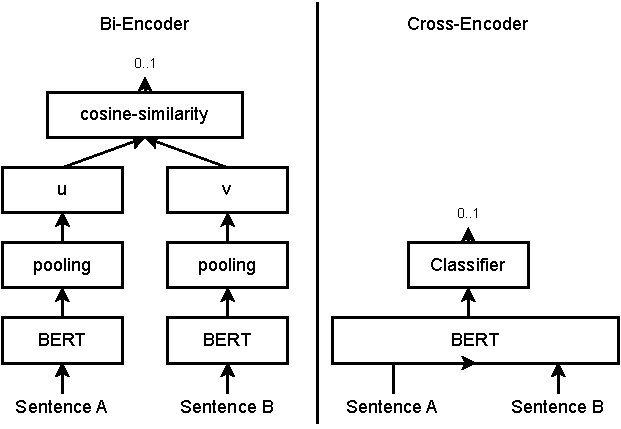
\includegraphics[width=.6\linewidth]{bivscross}
	\caption[Bi vs Cross-Encoder]{\label{fig:encoders}Bi vs Cross-Encoder. Taken from~\cite{sbert}.}
\end{figure}

\section{Normalized Discounted Cumulative Gain (NDCG)}\label{ndcg}

I will evaluate the different algorithms using the Normalized Discounted Cumulative Gain (NDCG). It is a standard quality measure often used for ranking recommendation systems that score the first k results compared to an ideal result.

We first need the gains for each ranking item to calculate the cumulative gain. These can be either manually assigned or created with a more performant model. These scores can be either clamped to 0 and 1 or continuous in that interval.

To calculate the cumulative gain (CG), we take the sum of all the individual gains up to the last rank k.

\[ CG = \sum_{i = 1}^{k} gains\]

This does not take into account the order of the results, so we discount the gains by rank to get the discounted cumulative gain (DCG).

\[ DCG = \sum_{i = 1}^{k} \frac{gains}{log_2(i+1)}\]

Lastly, we divide the discounted cumulative gain by the ideal discounted cumulative gain (IDCG), where everything is ranked in an optimal way to get the normalized discounted cumulative gain.

\[ NDCG = \frac{DCG}{IDCG}\]

Since the last rank k is crucial, we usually write NDCG@k, e.g., NDCG@10.

\section{Existing Datasets}

We can use existing datasets to fine-tune our models and to evaluate our search algorithms. There is no ready-made dataset for the pandas library, but potentially useful datasets include CodeSearchNet(NOTE:CITE), a dataset of functions and their docstrings, and the StackOverflow  data.

\chapter{Approach}\label{approach}

This chapter will go over my solution. My solution's three major building blocks are the recipes, the recommendation system, and the GUI. It will also go over the different ranking strategies in detail.

\section{Recipes}

Recipes are a data structure consisting of a code snippet, a description, a name, and optionally keywords or argument type information.

The name and description field should give the user information about what the recipe is for.
The code snippets themselves could be common functions for data manipulation, plotting, and data import and export.

The Recipes are implemented as a Python data class since they manage data, not logic.

\begin{listing}[htb]
\begin{minted}[frame=lines,
	framesep=2mm,
	baselinestretch=1.2,
	fontsize=\footnotesize,
	tabsize=4,
	linenos]{python}
# pandaRec/recipe.py

@dataclass
class Recipe:
	name: str
	description: str
	code: str
	keywords: str
\end{minted}
\caption{Recipe Dataclass.}
\end{listing}

The recipes are bundled into a dataset and saved inside a .json file, together with the dataset description and links to other resources I will discuss later. \label{jsonwhy}

There are multiple ways to generate these recipes. One could:

\begin{itemize}
	\item Generate recipes with the dir() method.
	\item Modify already existing snippets, e.g., from here:~\cite{basicpandassnippets}.
	\item Collect pandas usage data from publicly available sources (Stackoverflow, CodeSearchNet) and search for often used snippets.
	\item Create snippets from publicly available usage guides for pandas.
\end{itemize}

I used the first method to generate a basic set of recipes like this:

\begin{listing}[htb]
	\begin{minted}[
		frame=lines,
		framesep=2mm,
		baselinestretch=1.2,
		fontsize=\footnotesize,
		tabsize=4,
		linenos
		]{python}
# generate_recipes.ipynb

# modified from https://stackoverflow.com/a/34452
def get_methods(object):
	method_list = []
	for method in dir(object):
		# make sure its a function
		if not callable(getattr(object, method)):
			continue
		method_name = str(method)
		
		# ignore internal functions
		if method_name.startswith('_'):
			continue
		
		# only take functions with a docstring
		if str(getattr(object, method).__doc__) == 'None':
			continue
		method_list.append(
			[
				method_name,
				str(getattr(object, method).__doc__)
			]
		)
	return method_list

recipes = [
	Recipe(method[0], method[1].strip(), "df." + method[0], "")
	for method in get_methods(df)
]
	\end{minted}
	\caption{Generate Basic Recipes.}
\end{listing}

I also used the fourth method on the pandas documentation, specifically "10 minutes to pandas" and the "cookbook" from the pandas user guide (NOTE: cite link).

For the recipes I created, I followed the VSCode Snippet syntax for placeholder to make a later integration into VSCode easier. More on this in \Cref{futurework}.

\section{The Recommendation System}

\subsection{Context}

As described in~\Cref{coderecsystems}, the context is the system's input. My system collects the user query, along with the specified DataFrame and selections, rectangular areas in the DataFrame that the user selected.

\begin{listing}[htb]
	\begin{minted}[
		frame=lines,
		framesep=2mm,
		baselinestretch=1.2,
		fontsize=\footnotesize,
		tabsize=4,
		linenos
		]{python}
# pandaRec/context.py
from dataclasses import dataclass


@dataclass
class Selection:
	r1: int
	c1: int
	r2: int
	c2: int


class Context:
	selections: list[Selection]
	data: DataFrame
	query: str
	
	def __init__(...): ... # basic constructor, left out for brevity
	
	def is_whole_row(self, selection: Selection) -> bool:
		return selection.c1 == 0 and selection.c2 == self.data.shape[1]
	
	def is_whole_column(self, selection: Selection) -> bool:
		return selection.r1 == 0 and selection.r2 == self.data.shape[0]
	\end{minted}
	\caption{Context Class.}
\end{listing}

I also provide functions \mintinline[bgcolor=LightGray]{python}|is_whole_row()| and \mintinline[bgcolor=LightGray]{python}|is_whole_column()| so one can check whether a whole row/ column is selected.

\subsection{The Recommendation Engine}

My recommendation system uses a strategy pattern for the recommendation algorithm. This makes it easy to implement multiple algorithms.

The recommender class, therefore, only holds the context, the current recommend strategy, and the list of recipes.  Additionally, the strategy result is saved in the recommender as an ordered list of RecipeResults, recipes with scores.


\begin{listing}[htb]
\begin{minted}[
frame=lines,
framesep=2mm,
baselinestretch=1.2,
fontsize=\footnotesize,
tabsize=4,
linenos
]{python}
# pandaRec/recommender.py
class Recommender:
	context: Context
	search_algorithm: RecommendStrategy
	recipes: list[Recipe]
	recommended_recipes: list[RecipeResult]

	def __init__(...): ... # basic constructor, left out for brevity
	
	def recommend(self): # use the strategies search function
		self.recommended_recipes = self.search_algorithm.search(
			self.context, self.recipes
		)
	
	def show_results(self) -> str:
		result = ""
		for recipe_result in self.recommended_recipes:
			result +=
				f"{recipe_result.recipe.name}\t\tScore: {recipe_result.score}\n"
		return result
\end{minted}
\caption{Recommender Class\label{list:recommend}.}
\end{listing}

I decided not to save a reference to the index of the corresponding recipe inside the RecipeResults because, this way, a strategy can return arbitrary recipes. Storing the result list as a list of recipe indexes and score tuples would eliminate the data duplication, but I prefer the flexibility my approach provides.

\subsection{Ranking Strategies}

For my solution, I implemented multiple ranking strategies to compare them. These can be swapped out easily because of the strategy pattern.
\begin{listing}[htb]
\begin{minted}[
frame=lines,
framesep=2mm,
baselinestretch=1.2,
fontsize=\footnotesize,
tabsize=4,
linenos
]{python}
# pandaRec/strategies.py
from abc import ABC, abstractmethod

class RankingStrategy(ABC):
	@abstractmethod
	def search(self, context: Context, recipes: list[Recipe]) -> list[RecipeResult]:
		pass
\end{minted}
\caption{RankingStrategy Class.}
\end{listing}

Any strategy we add will inherit this abstract class and provide its search function. The recommender will call this function as shown in \Cref{list:recommend}. All my strategies score the recipes in the interval \( \left[0;1\right] \). Let us first look at a basic strategy to understand how this works.

\subsubsection{Name Search}

Name search searches for the query string in the name of the recipes, scoring it one if it finds it and not returning the recipe at all if the query string is absent. This ends up in name search working like code completion since the names of the auto-generated recipes are the same as the function names.

\begin{listing}[htb]
	\begin{minted}[
		frame=lines,
		framesep=2mm,
		baselinestretch=1.2,
		fontsize=\footnotesize,
		tabsize=4,
		linenos
		]{python}
# pandaRec/strategies.py
class NameSearch(RankingStrategy):
	@staticmethod
	def search(context: Context, recipes: list[Recipe]) -> list[RecipeResult]:
		result = []
		for recipe in recipes:
			if context.query in recipe.name:
			result.append(RecipeResult(1, recipe))
	return result
\end{minted}
\caption{Name Search.}
\end{listing}

We can see with this example how a ranking algorithm will work; it will iterate over the recipes, score them, sort them (not the case here since the scores are all 1), and then return them to the recommender.

\subsubsection{Fuzzy Search}

Fuzzy search uses a string distance function to search for approximately similar strings. The Levenshtein distance is commonly used. In it, the distance amount increases by a constant for every insertion, deletion, and substitution.

\begin{align}[htb]
lev(a, b) =
\begin{cases}
	|a| & \text{if } |b| = 0\\
	|b| & \text{if } |a| = 0\\
	lev(tail(a), tail(b)) & \text{if } a[0] == b[0]\\
	\min
	\begin{cases}
		lev(tail(a), b) &+ \text{ i}\\
		lev(a, tail(b)) &+ \text{ d}\\
		lev(tail(a), tail(b)) &+ \text{ c}
	\end{cases} & \text{else}
\end{cases}
\end{align}


If \(\text{i} + \text{d} = \text{c}\), this reduces to the InDel distance, which only counts insertions and deletions. Since performance starts to matter here, I have used the library "rapidfuzz" to calculate the distances. Their \mintinline[bgcolor=LightGray]{python}|partial_token_sort_ratio| function sorts the words and calculates the partial ratio between the prompt and the description.

(NOTE: funky code placement, fix after everything else is done)

\begin{listing}[htb]
	\begin{minted}[
		frame=lines,
		framesep=2mm,
		baselinestretch=1.2,
		fontsize=\footnotesize,
		tabsize=4,
		linenos
		]{python}
# pandaRec/strategies.py
class FuzzySearchDescription(RankingStrategy):
	def __init__(self, ratio=fuzz.partial_token_sort_ratio):
		super().__init__()
		self.ratio = ratio # let the user choose a different ratio if they want
	
	def search(self, context: Context, recipes: list[Recipe]) -> list[RecipeResult]:
		result = []
		for recipe in recipes:
			score = self.ratio(context.query, recipe.description,
			                   processor=default_process)
			result.append(RecipeResult(score, recipe))
		result.sort(key=lambda recipe_result: recipe_result.score, reverse=True)
		return result
		\end{minted}
	\caption{Fuzzy Search.}
\end{listing}

The partial ratio they use is implemented in C++ and runs for short queries (n<64), most queries will be this size, in worst-case O(nm) time, with m being the number of different alignments of the shorter string in the bigger string, effectively the size of the bigger string. Since we must iterate over all recipes, we get O(nmr), which can incur noticeable slowdowns (in the decisecond range) on web-hosted Jupyter engines. So, let us look at an algorithm that still allows us to find partial matches and matches of similar words while simultaneously being way faster.

\clearpage

\subsubsection{Index Search}

I have already introduced index search in \Cref{indexsearch}. We build the index when we construct the strategy, only if we do not provide a path to a prebuilt built index:

\begin{listing}[htb]
	\begin{minted}[
		frame=lines,
		framesep=2mm,
		baselinestretch=1.2,
		fontsize=\footnotesize,
		tabsize=4,
		highlightlines={6-8},
		linenos
		]{python}
# pandaRec/strategies.py
class IndexSearch(RankingStrategy):
	def __init__(self, recipes: list[Recipe], path: str = ""):
	super().__init__()
	if not path:
		self.index = generate_search_index(
			[recipe.description for recipe in recipes]
		)
	else:
		self.index = load_search_index(path)
	\end{minted}
	\caption{Index Search Constructor.}
\end{listing}

This path can be saved alongside the list of recipes in the .json and is one of the paths I alluded to in \Cref{jsonwhy}.

Before generating the index, we first want to lemmatize the descriptions (see~\Cref{lemmatize}). For this, we start by tokenizing the descriptions with the regex \mintinline[bgcolor=LightGray]{text}|"\w*[a-zA-Z]\w*"|, which matches words with at least one letter. We then use the Natural Language Toolkit NLTK to lemmatize the words and remove common stop words like "a" or "the" that are irrelevant to the search.

\begin{listing}[htb]
	\begin{minted}[
		frame=lines,
		framesep=2mm,
		baselinestretch=1.2,
		fontsize=\footnotesize,
		tabsize=4,
		linenos
		]{python}
# pandaRec/search_index.py
def lemmatize_no_stop_words(text: str) -> list[str]:
	words = re.findall(r"\w*[a-zA-Z]\w*", text)
	wnl = WordNetLemmatizer()
	return [
		wnl.lemmatize(word)
		for word in words
		if word not in stopwords.words("english")
		# stopwords are common words like "a" that are not relevant for the search
		]
	\end{minted}
	\caption{Lemmatization.}
\end{listing}

We can then build the forward index and, lastly, the inverted index.

\begin{listing}[htb]
	\begin{minted}[
		frame=lines,
		framesep=2mm,
		baselinestretch=1.2,
		fontsize=\footnotesize,
		tabsize=4,
		linenos
		]{python}
# pandaRec/search_index.py
def generate_search_index(descriptions: list[str])
		-> dict[str, list[tuple[int, int]]]:
	# 1. Lemmatize the descriptions
	lemmatized_descriptions = [
			lemmatize_no_stop_words(description) for description in descriptions
		]
	# 2. build the forward index, one list of (word, frequenzy) tuples
	# per description
	frequency_per_description = [
			[(word, description.count(word)) for word in set(description)]
			for description in lemmatized_descriptions
		]
	# 3. construct the inverted index as hashmap with list of
	# (description_index, frequency) tuples for each word
	frequency_per_word = {}
	for idx, description in enumerate(frequency_per_description):
		for (word, count) in description:
			if word not in frequency_per_word:
				frequency_per_word[word] = [(idx, count)]
			else:
				frequency_per_word[word].append((idx, count))
	return frequency_per_word
	\end{minted}
	\caption{Building the Inverted Index.}
\end{listing}

We can then pickle the hashmap to save it to disk.
When searching for a query, we lemmatize it and normalize how many query words are in each document.

\begin{listing}[htb]
	\begin{minted}[
		frame=lines,
		framesep=2mm,
		baselinestretch=1.2,
		fontsize=\footnotesize,
		tabsize=4,
		linenos
		]{python}
# pandaRec/strategies.py
class IndexSearch(RankingStrategy):
	...
	
	def search(self, context: Context, recipes: list[Recipe]) -> list[RecipeResult]:
		lemmatized_search = lemmatize_no_stop_words(context.query)
		
		# add 1 to the score for each word that is in the description (per recipe)
		scores = len(recipes) * [0]
		for word in lemmatized_search:
			if word in self.index:
				for idx, _ in self.index[word]:
					scores[idx] += 1
		
		num_words = len(lemmatized_search)
		result = [
				RecipeResult(score / num_words, recipe) # normalize score
				# scores and recipes are in the same order so we can zip() them
				for score, recipe in zip(scores, recipes) 
			]
		result.sort(key=lambda recipe_result: recipe_result.score, reverse=True)
		return result
\end{minted}
\caption{Searching the Inverted Index.}
\end{listing}

We also must sort the list of results since we want this list to be in the order of ranking.
\clearpage

\subsubsection{Semantic Search}

The basics of semantic search were already described in \Cref{semantic}. To implement a semantic search, we will use the Sentence-Transformers library, which is originally based on~\cite{reimers2019sentence}. Like constructing the reverse index in the index-based search, we first must create embeddings for all our recipes. This is again handled in the constructor.

\begin{listing}[htb]
	\begin{minted}[
		frame=lines,
		framesep=2mm,
		baselinestretch=1.2,
		fontsize=\footnotesize,
		tabsize=4,
		linenos
		]{python}
		# pandaRec/strategies.py
class SemanticSearch(RankingStrategy):
	def __init__(self, recipes: list[Recipe], path: str = "",
			     model: str = "sentence-transformers/all-mpnet-base-v2"):
	super().__init__()
	self.model = SentenceTransformer(model)
	descriptions = [recipe.description for recipe in recipes]
	if not path:
		self.embeddings = self.model.encode(descriptions)
	else:
		self.embeddings = load_embeddings(path)
	\end{minted}
	\caption{Embedding the Recipes.}
\end{listing}

We can then embed our query and use the cosine similarity to search for descriptions with similar semantic meanings. I have tested this algorithm with three different models: "all-mpnet-base-v2" and "all-MiniLM-L6-v2" which are general general-purpose, and "krlvi/sentence-t5-base-nlpl-code\_search\_net" which is trained with the "code\_search\_net" dataset (NOTE:cite). In \Cref{semanticmodels} I will evaluate the differences between these models.

\begin{listing}[htb]
	\begin{minted}[
		frame=lines,
		framesep=2mm,
		baselinestretch=1.2,
		fontsize=\footnotesize,
		tabsize=4,
		linenos
		]{python}
# pandaRec/strategies.py
class SemanticSearch(RankingStrategy):
	...
	
	def search(self, context: Context, recipes: list[Recipe]) -> list[RecipeResult]:
		query_embedding = self.model.encode(context.query, convert_to_tensor=True)
		cos_scores = [
			util.cos_sim(query_embedding, embedding).item(
			for embedding in self.embeddings
		]
		result = [
			RecipeResult(score, recipe)
			for recipe, score in zip(recipes, cos_scores)
		]
		result.sort(key=lambda recipe_result: recipe_result.score, reverse=True)
		return result

	\end{minted}
	\caption{Searching the Embeddings.\label{list:searchembed}}
\end{listing}
	
\subsubsection{OpenAI Embeddings}

We can also use OpenAIs API to generate embeddings. Their util function \mintinline[bgcolor=LightGray]{python}|get_embeddings| automatically manages batching, but the process is other than that the same as with Sentence-Transformers. The ranking process is the same as in \Cref{list:searchembed}.

\begin{listing}[htb]
	\begin{minted}[
		frame=lines,
		framesep=2mm,
		baselinestretch=1.2,
		fontsize=\footnotesize,
		tabsize=4,
		linenos
		]{python}
# pandaRec/strategies.py
class OpenAIEmbeddings(RankingStrategy):
	def __init__(
		self,
		recipes: list[Recipe],
		path: str = "",
		model: str = "text-embedding-ada-002",
	):
		super().__init__()
		self.model = model
		descriptions = [recipe.description for recipe in recipes]
		if not path:
			self.embeddings = get_embeddings(descriptions, engine=self.model)
		else:
			self.embeddings = load_embeddings(path)
\end{minted}
\caption{OpenAI embeddings.}
\end{listing}


\clearpage

\section{The Jupyter Notebook GUI}

For my solution, I decided to go with a Jupyter Notebook GUI. Jupyter Notebooks are already used extensively in machine learning and data science since they have many essential strengths in these fields. Being able to run code cell-by-cell, one can quickly explore and visualize data. The capability to render markdown also helps with documentation. Lastly, services like google colab allow for running notebooks directly in the browser without extensive setup.

(NOTE: Maybe change to a screenshot that shows off the code field better)

\begin{figure}[htb]
	\centering
	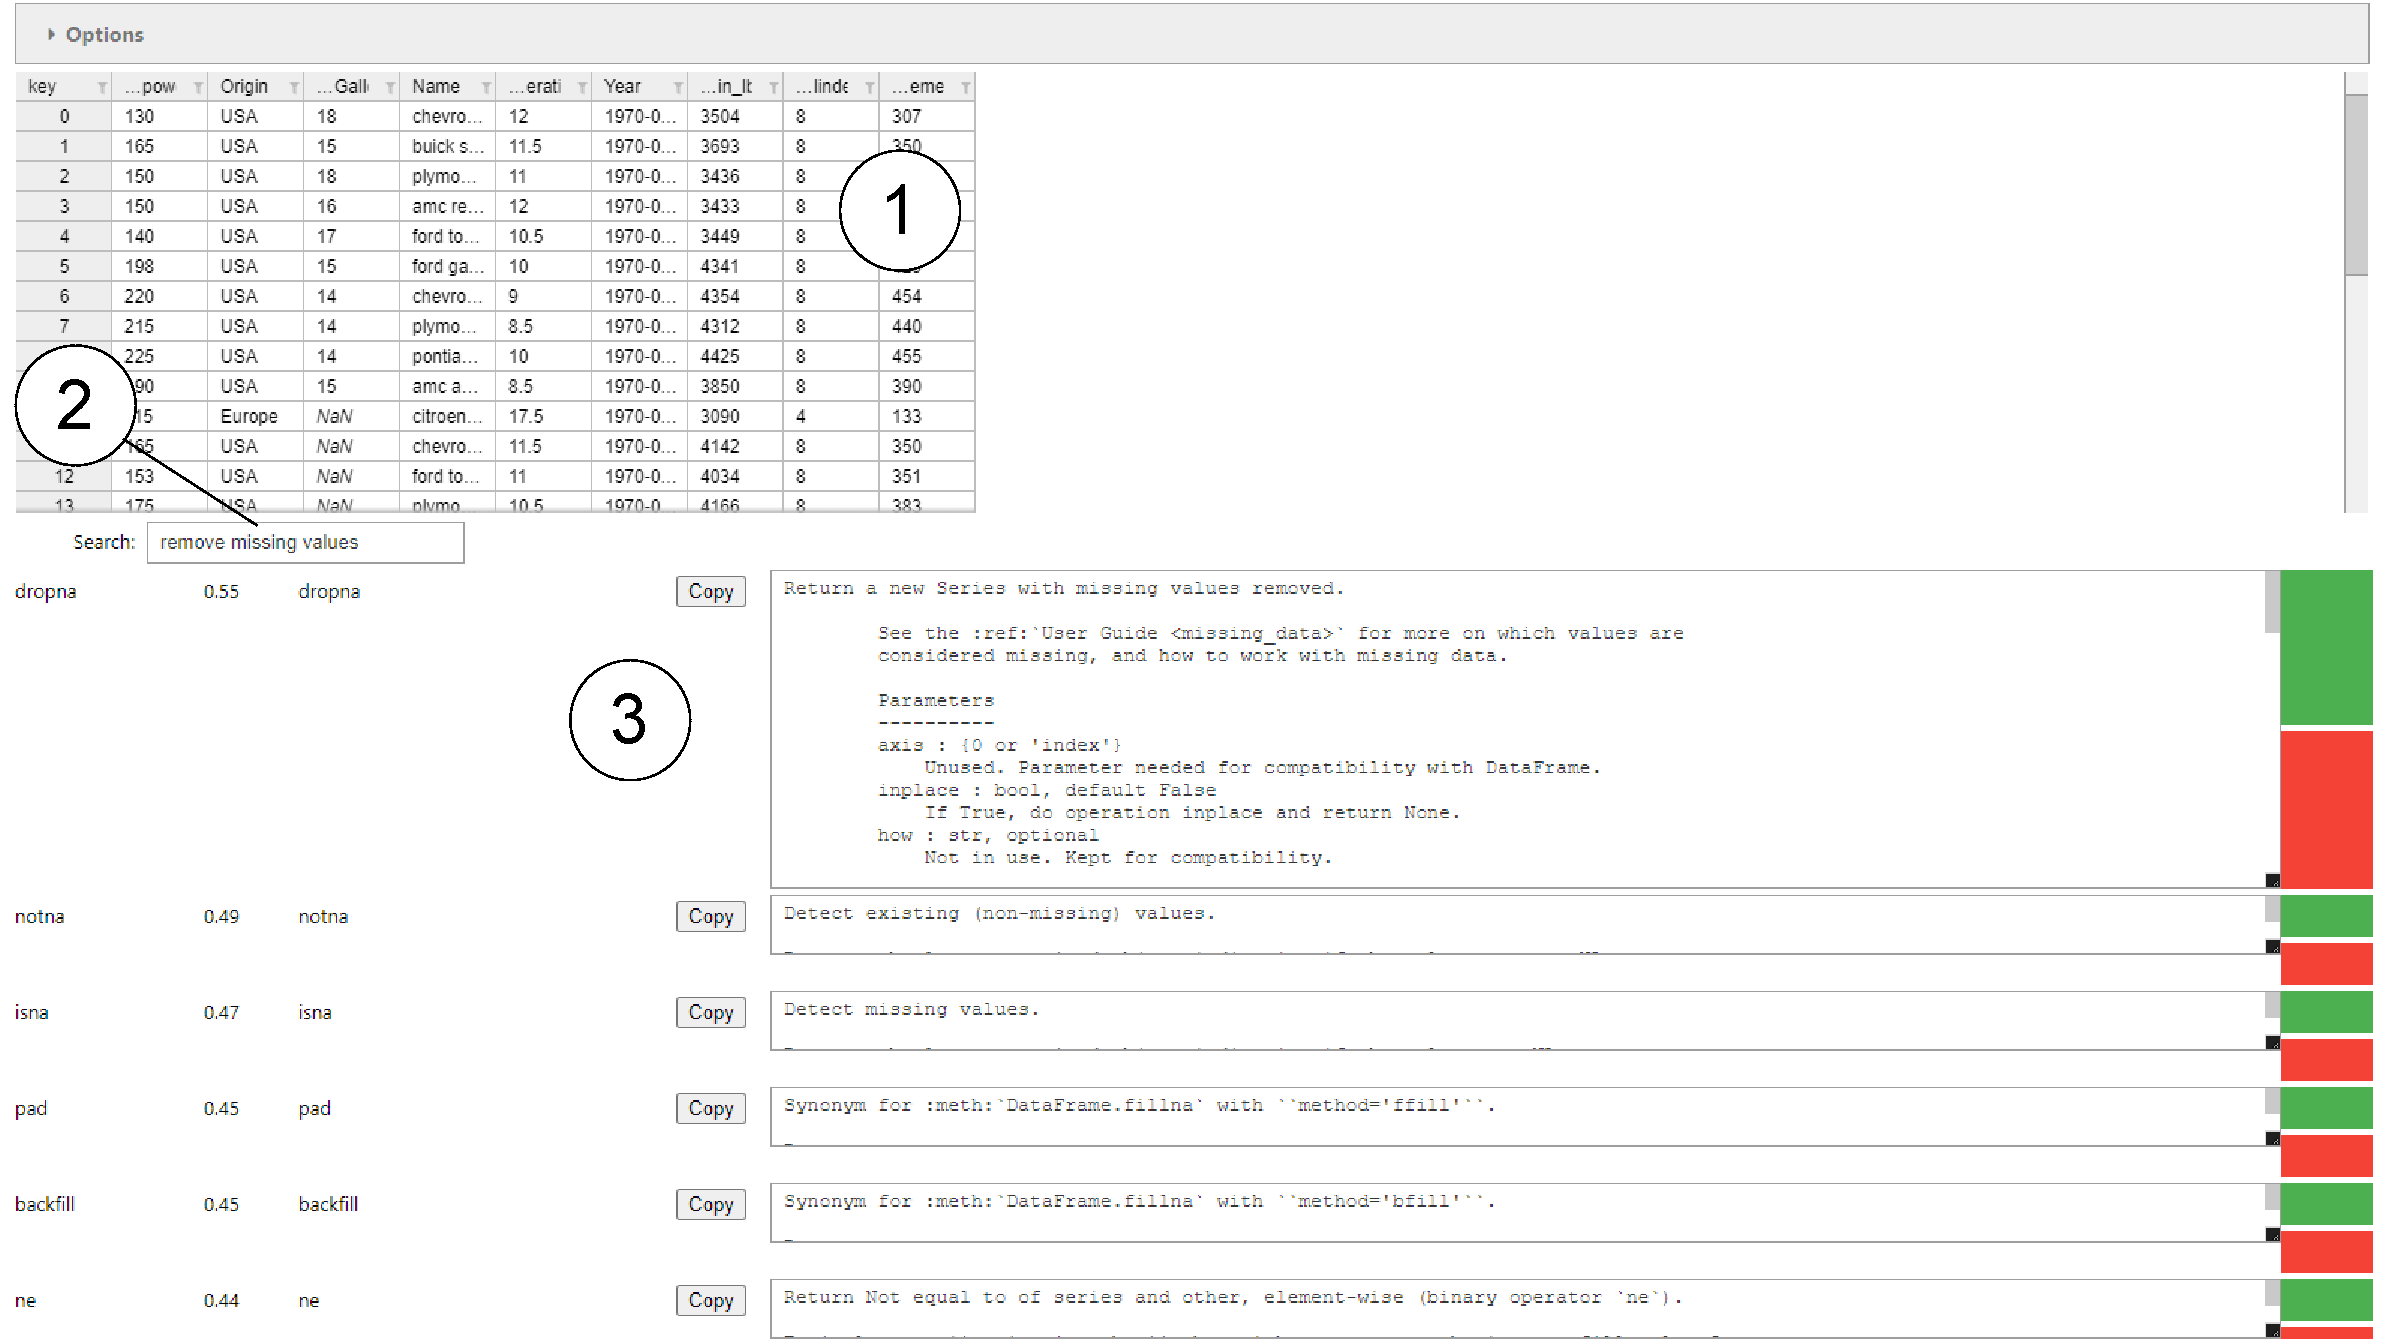
\includegraphics[width=\linewidth]{widget_annotated}
	\caption[Recommender Widget]{\label{fig:encoders}Main parts of the recommender.}
\end{figure}

The GUI is made of three main building blocks:

\begin{enumerate}
	\item The data grid.
	\item The search box.
	\item The search results.
\end{enumerate}

There also exists an options dropdown menu.

\subsection{The Data Grid and Search Box}

The data grid uses the library ipydatagrid(NOTE:cite), a data grid widget that is recommended by the Jupyter Tutorial(NOTE:cite). It allows for scrolling, resizing, and selecting, which is more than enough for our use case.

The search box is a Text widget.

\subsection{The Search Results}

The search results are shown in a vertical list. Each result has, in order, a name, score, code snippet, copy button, and description. The descriptions are resizable to allow for longer descriptions. The user can change the length of the list in the options.

\subsection{Updating Results}

To update the results, I used the observe methods of the various widgets to register a callback.

\begin{listing}[htb]
	\begin{minted}[
		frame=lines,
		framesep=2mm,
		baselinestretch=1.2,
		fontsize=\footnotesize,
		tabsize=4,
		linenos
		]{python}
		# pandaRec/panda_rec_widget.py
		class PandaRecWidget(widgets.VBox):
		def __init__(...):
		...
		self.search_box.observe(self.update_recommendations, names="value")
		self.data_grid.observe(self.update_recommendations, names="selected_cells")
		
		def update_recommendations(self, _change):
		self.recommender.set_search(str(self.search_box.value))
		self.recommender.set_selection(self.data_grid.selected_cells)
		self.recommender.recommend()
		self.result_widget.update(self.recommender.recommended_recipes)
	\end{minted}
	\caption{Observe Callbacks.}
\end{listing}

This callback then updates the context of the recommender, recommends recipes, and changes the search results. There is a consideration here about whether we want the callback to be triggered anytime a change is made or only after a short duration of inactivity. This could result in additional costs, especially for the OpenAI Embeddings since we send more requests than necessary. I decided not to implement this since, as we will see, all algorithms are quick. If needed, however, one could follow the Jupyter Widgets Documentation to create a debouncing decorator(NOTE:cite). (NOTE: I did this by now, update)

\subsection{Applying the Code Snippet}

We could apply code snippets to the underlying DataFrame in two main ways. We could use \mintinline[bgcolor=LightGray]{python}|eval()| to directly evaluate the code snippet or copy it to a new cell directly or via user input. The \mintinline[bgcolor=LightGray]{python}|eval()| approach makes changing, e.g., row names before evaluating, more complicated and will also lose Jupyter notebooks upside of cell-by-cell execution. By copying the snippet to the clipboard, we allow the user to choose what to do with it.

When using the notebook online, we cannot easily access the clipboard with the Pyperclip library. That is why I created a copy button with \mintinline[bgcolor=LightGray]{python}|ipywidgets.HTML|, which allows for custom HTML input.

\begin{listing}[htb]
	\begin{minted}[
		frame=lines,
		framesep=2mm,
		baselinestretch=1.2,
		fontsize=\footnotesize,
		tabsize=4,
		linenos
		]{python}
# pandaRec/copybutton.py
import ipywidgets as widgets

def copy_button_html(copytext=""):
	base_html = """
	<button class="copybutton" onclick=navigator.clipboard.writeText('{}')>
		Copy
	</button>
	"""
	return base_html.format(copytext)

	\end{minted}
	\caption{Copy Button.}
\end{listing}

\chapter{Evaluation}\label{evaluation}

This chapter evaluates the different ranking algorithms concerning their setup speed, search speed, and ranking performance. It will also compare the different recipe datasets.

\section{Setup and Search Delays}

To evaluate delays in the system, we can use Jupyter notebooks inbuild \%timeit magic command, which uses the timeit module to time the execution of a statement. As an example, this is what timing the setup time for index search with a saved index looks like:

\begin{listing}[htb]
	\begin{minted}[
		frame=lines,
		framesep=2mm,
		baselinestretch=1.2,
		fontsize=\footnotesize,
		tabsize=4,
		linenos
		]{python}
%timeit IndexSearch(recipes, '../recipes/search_index.pkl')

# 1.50 ms ± 3.07 µs per loop (mean ± std. dev. of 7 runs, 1,000 loops each)
	\end{minted}
	\caption{Timing index search with a saved index.}
\end{listing}

If we do this for all implemented algorithms, we can compare their setup and search time. I have used the query "fill missing values with zero" to analyze search time.


\begin{table}[htb]
	\centering
\begin{tabular}{l S S}
	\toprule
	Name                     & {Setup Time}                   & {Search Time}                  \\ \midrule
	Name Search              & \SI{68(0.2)}{\nano\second}     & \SI{6.53(0.08)}{\micro\second} \\
	Fuzzy Name Search        & \SI{68.4(0.5)}{\nano\second}   & \SI{756(1.3)}{\micro\second}   \\
	Fuzzy Description Search & \SI{276(0.8)}{\nano\second}    & \SI{10(0.05)}{\milli\second}   \\
	Index Search             & \SI{7.87(0.08)}{\second}       & \SI{1.74(0.01)}{\milli\second} \\
	Semantic Search          & \SI{85(1)}{\second}            & \SI{38.2(0.9)}{\milli\second}  \\
	OpenAI Embedding         & \SI{3(1)}{\second}             & \SI{668(949)}{\milli\second}   \\ \midrule
	\multicolumn{3}{l}{Saved Index/ Embedding}                                                 \\ \midrule
	Index Search             & \SI{1.5(0.03)}{\milli\second}  & {-}                            \\
	Semantic Search          & \SI{682(10)}{\milli\second}    & {-}                            \\
	OpenAI Embedding         & \SI{27.5(0.25)}{\milli\second} & {-}                            \\ \bottomrule
\end{tabular}
\caption[Search Delay]{\label{tab:delay}Setup and search delay for all implemented algorithms.}
\end{table}

Name search and fuzzy name search both do not have any setup, and fuzzy description search only registers the fuzzy ratio algorithm, which results in basically instant setup time. Index search takes about 8 seconds to build the index.
The embedding using Sentence Transformers takes about one and a half minutes to embed all the descriptions. This could be sped up by using the GPU by passing \mintinline[bgcolor=LightGray]{python}|device="cuda"| to the SentenceTransformer constructor. The OpenAI Embedding is batched and calculated remotely, which should keep the setup time decoupled from the hardware.

\section{Algorithm Accuracy}

To evaluate the accuracy of the algorithms, we will use the NDCG introduced in \Cref{ndcg}.

\subsection{Creating the Ranking Dataset}

There are no good pre-existing datasets for ranking the algorithms, so I will create my own. To do this, I selected the article (NOTE: cite article). For every one of the thirty functions, I created a description and selected recipes that can fulfill these goals (NOTE: weird wording), which I assigned the score one. I then calculated the NDCG@5 for each of the algorithms. For some of the descriptions, none of the recipes can fulfill the goal. These are not counted towards the NDCG@5 score (since the IDCG@5 is 0, breaking our formula). Here is an overview of how many of the descriptions cannot be achieved by each recipe dataset:

(NOTE: Table of nonachievements)

\subsection{Ranking Based on the Autogenerated Recipes}

Since none of the ranking descriptions are substrings of the recipes' names, Name Search does not recommend anything and, therefore, always scores zero. This is fine since it worked more as a proof of concept, but I will omit it in the following tables.

I was expecting both the lexical searches and the embeddings to work well on the autogenerated recipes since they have a decently long description, with a mean length of 2221 characters and a mean amount of 71.6 lines.


\begin{table}[htb]
	\centering
	\begin{tabular}{l S}
		\toprule
		Name                     & {Score} \\ \midrule
		Name Search              & 0       \\
		Fuzzy Name Search        & 0.39    \\
		Fuzzy Description Search & 0.26    \\
		Index Search             & 0.21    \\
		Semantic Search          & 0.62    \\
		OpenAI Embedding         & 0.54    \\ \bottomrule
	\end{tabular}
	\caption[NDCG Scores]{\label{tab:ndcg}NDCG Scores for all implemented algorithms.}
\end{table}

The Lexical search algorithms work noticably (NOTE:finish)

\subsection{Comparing Semantic Search Models\label{semanticmodels}}

Now, let us compare the different models I considered for the semantic search using Sentence-Transformers.

\begin{description}
	\item[all-mpnet-base-v2] is the general-purpose model from Sentence-Transformers with the best quality.
	\item[all-MiniLM-L6-v2] is a smaller general-purpose model that the Sentence-Transformer documentation claims is five times faster at the cost of some performance.
	\item[sentence-t5-base] is the base model of the t5 architecture, which is trained on predicting multiple masked words simultaneously. 
	\item[krlvi/sentence-t5-base-nlpl-code\_search\_net] is based on a t5-base checkpoint and trained on the "code\_search\_net" dataset.
\end{description}

\begin{table}[htb]
	\centering
	\begin{tabular}{l S S S}
		\toprule
		Name                   & {Score} & {Setup Delay}            & {Search Delay}                \\ \midrule
		all-mpnet-base-v2      & 0.62    & \SI{85 (1)}{\second}     & \SI{38.2(0.9)}{\milli\second} \\
		all-MiniLM-L6-v2       & 0.50    & \SI{10.3 (0.1)}{\second} & \SI{16.4(0.6)}{\milli\second} \\
		sentence-t5-base       & 0.53    & \SI{52.3 (0.5)}{\second} & \SI{40.6(9.2)}{\milli\second} \\
		sentence-t5-base-\dots & 0.48    & \SI{50.8 (0.5)}{\second} & \SI{39.6(1.1)}{\milli\second} \\ \bottomrule
	\end{tabular}
	\caption[NDCG Scores]{\label{tab:ndcg}NDCG Scores for different models.}
\end{table}

Using all-MiniLM-L6-v2 resulted in a $8.3\times$ speedup in setup delay and a $2.3\times$ speedup in searching delay. The model trained on "code\_search\_net" is noticeably worse than even. This is confirmation that the "code\_search\_net" will not help much in training a good model.

\subsection{Performance of the Different Recipe Datasets}

ranking different recipe datasets (NOTE: do this)

\section{Working With Jupyter Notebooks}



I decided to implement my solution in Jupyter Notebooks. Notebooks in combination with 

\subsection{Observing the DataFrame}

When we change the DataFrame with either a copied function or, in general, we would like to automatically update the recommender's DataFrame and the data grid. However, this is currently not supported by the widgets library (CITE:https://github.com/bloomberg/ipydatagrid/issues/6).

reflection: no observe on dataframes

outlook: fine-tune, use 


(NOTE: copy results from notebook to here)

bad: no observe on dataframes

\chapter{Conclusion}

\section{Future Work}\label{futurework}

semantic search + documentation = good combo
future work: fine tuning and adding NL based on row/ line names
\cite{wang2021gpl}
\cite{wang2021tsdae}
\cite{gao2021simcse}
porting to vscode
implementing a more advanced web based algorithm

\printbibliography

\end{document}
